	\begin{myprop}
	Si le point $B$ est le symétrique du point $A$ par rapport à une droite $(d)$, alors la droite $(d)$ est la médiatrice du segment $[AB]$.
\end{myprop}

\begin{mymeth}
	Pour tracer le symétrique d'un point $A$ par rapport à une droite $(d)$ :
	
	
	\begin{enumerate}
		%	\begin{multicols}{3}
		
		
		\item  On fixe un écartement de notre compas suffisamment grand. On pique en A et on trace deux arcs de cercle qui coupe la droite $(d)$ en deux endroits.
		
		\begin{center}
			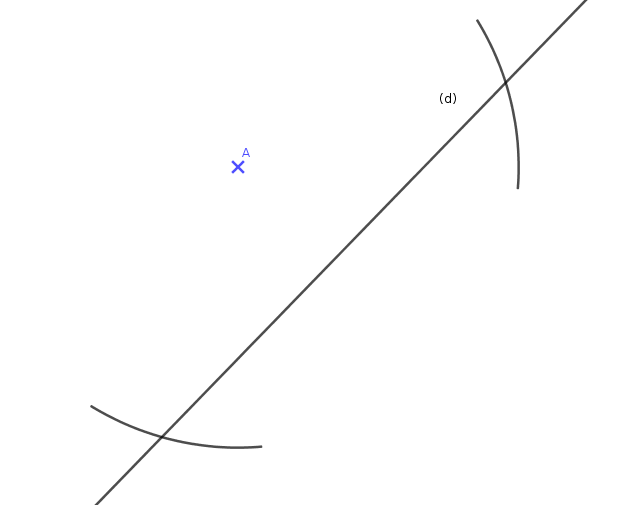
\includegraphics[scale=0.2]{meth1}
		\end{center}
		
		
		\item Toujours avec le même écartement. On pique au niveau de la première intersection et on créé un arc de cercle de l'autre côté de la droite $(d)$.
		
		\begin{center}
			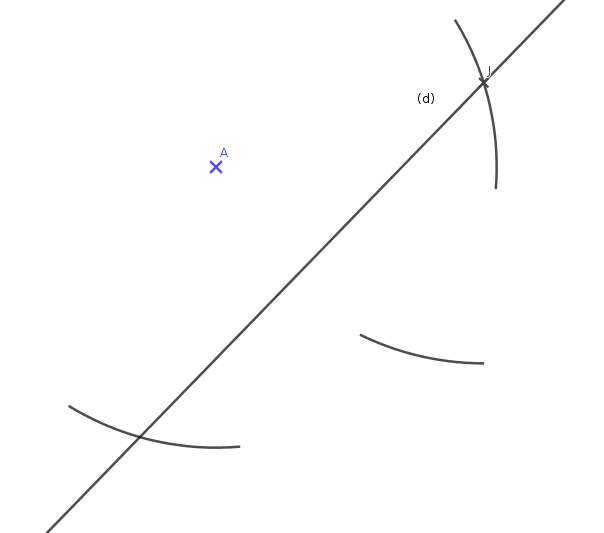
\includegraphics[scale=0.2]{meth2}
		\end{center}
		\item Toujours avec le même écartement. On pique au niveau de la 2$^e$ intersection et on créé un arc de cercle de l'autre côté de la droite $(d)$ qui va couper le dernier arc de cercle tracé, le point d'intersection est le symétrie de $A$.
		
		\begin{center}
			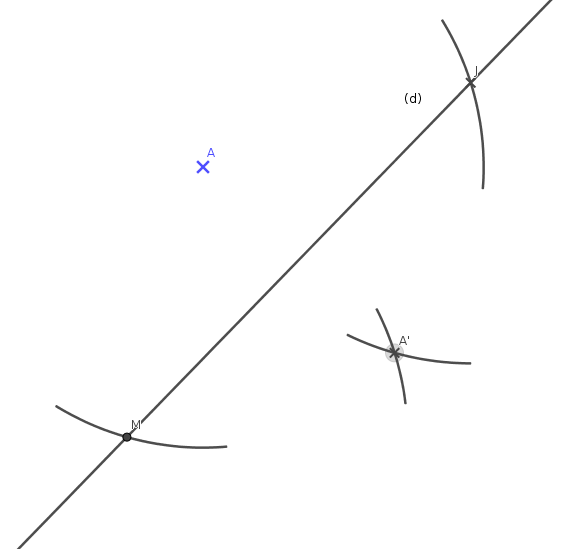
\includegraphics[scale=0.2]{meth3}
		\end{center}
		
		%	\end{multicols}
	\end{enumerate}
\end{mymeth}